\subsection{Pure \ch{NO} measurements with synthetic air}
\label{sec:no}

After confirming that our generator produced a clean ozone stream, we
turned towards the question whether it is possible to actually measure
\ch{NO} or not. Furthermore we wanted to get an estimate for the
necessary reaction pathlength as computed in
Section~\ref{sec:requirements}.

\subsubsection{Setup}
\label{sec:no-setup}

In order to be able to measure the nitrogen monoxide concentration
directly without additional corrections and computations, we had to
make sure that the used sample air was nitrogen dioxide free. This
lead us to the setup depicted in Figure~\ref{fig:no-setup}. We used
synthetic air and \ch{NO} calibration gas with a known \ch{NO}
concentration ($c = \SI{8.177}{ppm}$) together with a mass flow
controller to generate synthetic sample air with a precisely known
\ch{NO} concentration. In order to minimize the influence on the
pressure inside the cavity, we decided to overflow the air inlet
instead of bypassing the cavity pump as is done during a Helium
calibration. Thus we set the synthetic air flow to $\Phi_{\text{air}}$
to \SI{3}{\liter\per\minute}. The cavity itself was in the standard
setup described in Section~\ref{sec:inclusion}, except for the
reaction tube length which was varied between \SI{5}{\meter},
\SI{10}{\meter} and \SI{15}{\meter}. For each of these lengths we
varied the \ch{NO} calibration gas flow between \num{0} and
\SI{0.03}{\liter\per\minute}. As zero air we used ambient lab air
together with a zero air cartridge.

\begin{figure}[htbp]
  \centering
  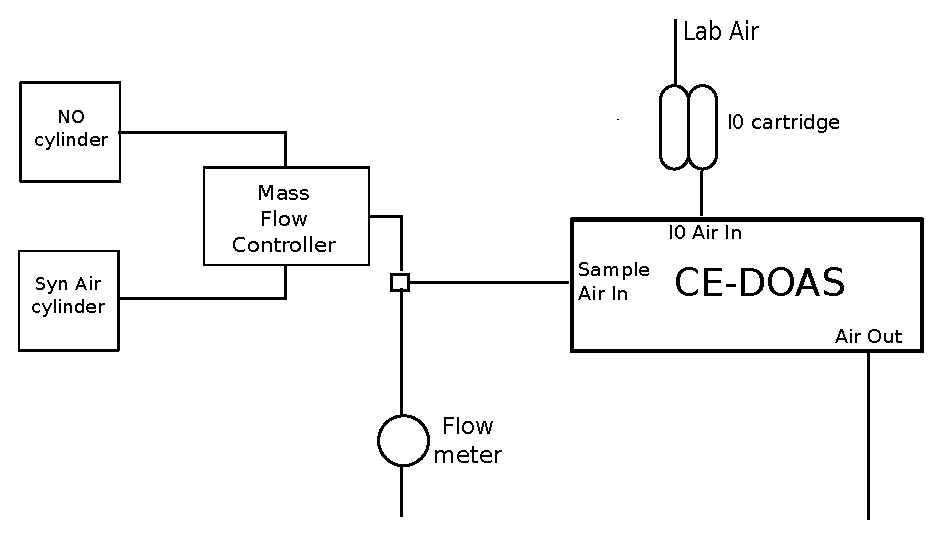
\includegraphics[width=0.6\textwidth]{no_setup.eps}
  \caption{Setup of the calibration measurement}
  \label{fig:no-setup}
\end{figure}

In order to be able to compare the measured \ch{NO} concentration to the
actual concentration in the air stream, we had to convert the applied
\ch{NO} flow to a concentration, too. We were able to do this using the
following formula
\begin{align}
  c_{\ch{NO}} = c \cdot \frac{\Phi_{\ch{NO}}}{\Phi_{\text{air}} +
  \Phi_{\ch{NO}}}. \label{eq:c-flow}
\end{align}

\subsubsection{Results}
\label{sec:no-results}

Figure~\ref{fig:ts} shows the time series of the \ch{NO} and \ch{O3}
concentration. Each of the three clusters corresponds from left to
right to the reaction tube length of \SI{5}{\meter}, \SI{10}{\meter}
and \SI{15}{\meter}. Turning first towards the ozone concentration on
the right hand side, we see that its concentration is constant within
its error margins. These, however, are large. This is to be expected,
as the absorption cross section of \ch{O3} in the visual spectrum is
weak compared to the cross section of \ch{NO2} and has almost no
differential structure. Nevertheless, the ozone level seems acceptably
stable, which indicates that not too many ozone destroying reactions
take place, even in the presence of high \ch{NO} concentrations. This
is again what we expected in this very pure sample air which should
only allow for the oxidation of \ch{NO}. Lastly the shape of the ozone
time series does not seem to depend on the reaction pathlength.

Looking at the \ch{NO} time series on the right hand side of
Figure~\ref{fig:ts} we see that the overall shape of the three
measurements are similar. For the reaction tube length of $l=
\SI{5}{\meter}$ we see slight deviations. The rising flanks take
longer to reach a stable plateau than during the other two
measurements. Furthermore the first three plateaus are not visible,
however, the reason for this lies in the fact that they were skipped
during the measurement procedure. The behaviour of the rising flanks
cannot simply be explained by a too short reaction path. If this were
the case, the depcited equilibria should all just lay lower, as the
reaction dynamic equilibrium would set for a lower, but
\emph{constant} \ch{NO2} concentration. Interstingly on the falling
flanks the equilibria are reached instantaneously (the small drop at
\SI{50}{ppb} being a human error). One possible explanation might lie
in the adsorption behaviour of teflon. For example if the ozone were
to be adsorbed to the tube walls, this could lead to an effective
increase in ozone concentration, accelerating the reaction and thus
compensating the too short pathlength. If, additionally, the
adsorption time scale were in the order of magnitude of our dwell time
per set flow, this could explain why we have slowly increasing flanks,
while the falling flanks stabilize quickly. In the first case the
adsorbed ozone would have to build up, because of the increased
concentration, in the second case there would already be enough ozone
adsorbed. The testing of this idea was sadly outside the scope of this
thesis, such that for the following measurements we could only accept
this oddity and decided to work with longer pathlengths (i.\,e.~$l =
\SI{10}{\meter}$) which seem to not express this behaviour.

\begin{figure}[htbp]
  \centering
  % GNUPLOT: LaTeX picture with Postscript
\begingroup
  \makeatletter
  \providecommand\color[2][]{%
    \GenericError{(gnuplot) \space\space\space\@spaces}{%
      Package color not loaded in conjunction with
      terminal option `colourtext'%
    }{See the gnuplot documentation for explanation.%
    }{Either use 'blacktext' in gnuplot or load the package
      color.sty in LaTeX.}%
    \renewcommand\color[2][]{}%
  }%
  \providecommand\includegraphics[2][]{%
    \GenericError{(gnuplot) \space\space\space\@spaces}{%
      Package graphicx or graphics not loaded%
    }{See the gnuplot documentation for explanation.%
    }{The gnuplot epslatex terminal needs graphicx.sty or graphics.sty.}%
    \renewcommand\includegraphics[2][]{}%
  }%
  \providecommand\rotatebox[2]{#2}%
  \@ifundefined{ifGPcolor}{%
    \newif\ifGPcolor
    \GPcolorfalse
  }{}%
  \@ifundefined{ifGPblacktext}{%
    \newif\ifGPblacktext
    \GPblacktexttrue
  }{}%
  % define a \g@addto@macro without @ in the name:
  \let\gplgaddtomacro\g@addto@macro
  % define empty templates for all commands taking text:
  \gdef\gplbacktext{}%
  \gdef\gplfronttext{}%
  \makeatother
  \ifGPblacktext
    % no textcolor at all
    \def\colorrgb#1{}%
    \def\colorgray#1{}%
  \else
    % gray or color?
    \ifGPcolor
      \def\colorrgb#1{\color[rgb]{#1}}%
      \def\colorgray#1{\color[gray]{#1}}%
      \expandafter\def\csname LTw\endcsname{\color{white}}%
      \expandafter\def\csname LTb\endcsname{\color{black}}%
      \expandafter\def\csname LTa\endcsname{\color{black}}%
      \expandafter\def\csname LT0\endcsname{\color[rgb]{1,0,0}}%
      \expandafter\def\csname LT1\endcsname{\color[rgb]{0,1,0}}%
      \expandafter\def\csname LT2\endcsname{\color[rgb]{0,0,1}}%
      \expandafter\def\csname LT3\endcsname{\color[rgb]{1,0,1}}%
      \expandafter\def\csname LT4\endcsname{\color[rgb]{0,1,1}}%
      \expandafter\def\csname LT5\endcsname{\color[rgb]{1,1,0}}%
      \expandafter\def\csname LT6\endcsname{\color[rgb]{0,0,0}}%
      \expandafter\def\csname LT7\endcsname{\color[rgb]{1,0.3,0}}%
      \expandafter\def\csname LT8\endcsname{\color[rgb]{0.5,0.5,0.5}}%
    \else
      % gray
      \def\colorrgb#1{\color{black}}%
      \def\colorgray#1{\color[gray]{#1}}%
      \expandafter\def\csname LTw\endcsname{\color{white}}%
      \expandafter\def\csname LTb\endcsname{\color{black}}%
      \expandafter\def\csname LTa\endcsname{\color{black}}%
      \expandafter\def\csname LT0\endcsname{\color{black}}%
      \expandafter\def\csname LT1\endcsname{\color{black}}%
      \expandafter\def\csname LT2\endcsname{\color{black}}%
      \expandafter\def\csname LT3\endcsname{\color{black}}%
      \expandafter\def\csname LT4\endcsname{\color{black}}%
      \expandafter\def\csname LT5\endcsname{\color{black}}%
      \expandafter\def\csname LT6\endcsname{\color{black}}%
      \expandafter\def\csname LT7\endcsname{\color{black}}%
      \expandafter\def\csname LT8\endcsname{\color{black}}%
    \fi
  \fi
    \setlength{\unitlength}{0.0500bp}%
    \ifx\gptboxheight\undefined%
      \newlength{\gptboxheight}%
      \newlength{\gptboxwidth}%
      \newsavebox{\gptboxtext}%
    \fi%
    \setlength{\fboxrule}{0.5pt}%
    \setlength{\fboxsep}{1pt}%
\begin{picture}(4030.00,4030.00)%
    \gplgaddtomacro\gplbacktext{%
      \csname LTb\endcsname%
      \put(682,686){\makebox(0,0)[r]{\strut{}$0$}}%
      \put(682,984){\makebox(0,0)[r]{\strut{}$10$}}%
      \put(682,1282){\makebox(0,0)[r]{\strut{}$20$}}%
      \put(682,1580){\makebox(0,0)[r]{\strut{}$30$}}%
      \put(682,1878){\makebox(0,0)[r]{\strut{}$40$}}%
      \put(682,2177){\makebox(0,0)[r]{\strut{}$50$}}%
      \put(682,2475){\makebox(0,0)[r]{\strut{}$60$}}%
      \put(682,2773){\makebox(0,0)[r]{\strut{}$70$}}%
      \put(682,3071){\makebox(0,0)[r]{\strut{}$80$}}%
      \put(682,3369){\makebox(0,0)[r]{\strut{}$90$}}%
      \put(814,554){\rotatebox{-45}{\makebox(0,0)[l]{\strut{}16:00}}}%
      \put(1096,554){\rotatebox{-45}{\makebox(0,0)[l]{\strut{}17:00}}}%
      \put(1378,554){\rotatebox{-45}{\makebox(0,0)[l]{\strut{}18:00}}}%
      \put(1660,554){\rotatebox{-45}{\makebox(0,0)[l]{\strut{}19:00}}}%
      \put(1942,554){\rotatebox{-45}{\makebox(0,0)[l]{\strut{}20:00}}}%
      \put(2224,554){\rotatebox{-45}{\makebox(0,0)[l]{\strut{}21:00}}}%
      \put(2505,554){\rotatebox{-45}{\makebox(0,0)[l]{\strut{}22:00}}}%
      \put(2787,554){\rotatebox{-45}{\makebox(0,0)[l]{\strut{}23:00}}}%
      \put(3069,554){\rotatebox{-45}{\makebox(0,0)[l]{\strut{}00:00}}}%
      \put(3351,554){\rotatebox{-45}{\makebox(0,0)[l]{\strut{}01:00}}}%
      \put(3633,554){\rotatebox{-45}{\makebox(0,0)[l]{\strut{}02:00}}}%
    }%
    \gplgaddtomacro\gplfronttext{%
      \csname LTb\endcsname%
      \put(176,2027){\rotatebox{-270}{\makebox(0,0){\strut{}Concentration [ppb]}}}%
      \put(2223,3699){\makebox(0,0){\strut{}Nitrogen Dioxide}}%
    }%
    \gplbacktext
    \put(0,0){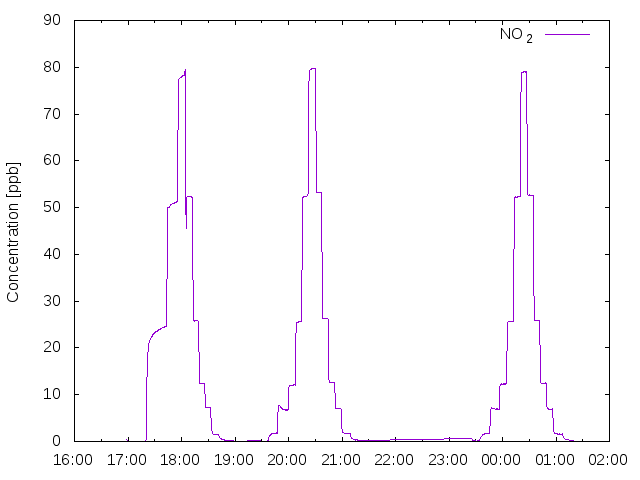
\includegraphics{../images/20160222_NO_fixI0_NO_ts}}%
    \gplfronttext
  \end{picture}%
\endgroup

  \hfill
  % GNUPLOT: LaTeX picture with Postscript
\begingroup
  \makeatletter
  \providecommand\color[2][]{%
    \GenericError{(gnuplot) \space\space\space\@spaces}{%
      Package color not loaded in conjunction with
      terminal option `colourtext'%
    }{See the gnuplot documentation for explanation.%
    }{Either use 'blacktext' in gnuplot or load the package
      color.sty in LaTeX.}%
    \renewcommand\color[2][]{}%
  }%
  \providecommand\includegraphics[2][]{%
    \GenericError{(gnuplot) \space\space\space\@spaces}{%
      Package graphicx or graphics not loaded%
    }{See the gnuplot documentation for explanation.%
    }{The gnuplot epslatex terminal needs graphicx.sty or graphics.sty.}%
    \renewcommand\includegraphics[2][]{}%
  }%
  \providecommand\rotatebox[2]{#2}%
  \@ifundefined{ifGPcolor}{%
    \newif\ifGPcolor
    \GPcolorfalse
  }{}%
  \@ifundefined{ifGPblacktext}{%
    \newif\ifGPblacktext
    \GPblacktexttrue
  }{}%
  % define a \g@addto@macro without @ in the name:
  \let\gplgaddtomacro\g@addto@macro
  % define empty templates for all commands taking text:
  \gdef\gplbacktext{}%
  \gdef\gplfronttext{}%
  \makeatother
  \ifGPblacktext
    % no textcolor at all
    \def\colorrgb#1{}%
    \def\colorgray#1{}%
  \else
    % gray or color?
    \ifGPcolor
      \def\colorrgb#1{\color[rgb]{#1}}%
      \def\colorgray#1{\color[gray]{#1}}%
      \expandafter\def\csname LTw\endcsname{\color{white}}%
      \expandafter\def\csname LTb\endcsname{\color{black}}%
      \expandafter\def\csname LTa\endcsname{\color{black}}%
      \expandafter\def\csname LT0\endcsname{\color[rgb]{1,0,0}}%
      \expandafter\def\csname LT1\endcsname{\color[rgb]{0,1,0}}%
      \expandafter\def\csname LT2\endcsname{\color[rgb]{0,0,1}}%
      \expandafter\def\csname LT3\endcsname{\color[rgb]{1,0,1}}%
      \expandafter\def\csname LT4\endcsname{\color[rgb]{0,1,1}}%
      \expandafter\def\csname LT5\endcsname{\color[rgb]{1,1,0}}%
      \expandafter\def\csname LT6\endcsname{\color[rgb]{0,0,0}}%
      \expandafter\def\csname LT7\endcsname{\color[rgb]{1,0.3,0}}%
      \expandafter\def\csname LT8\endcsname{\color[rgb]{0.5,0.5,0.5}}%
    \else
      % gray
      \def\colorrgb#1{\color{black}}%
      \def\colorgray#1{\color[gray]{#1}}%
      \expandafter\def\csname LTw\endcsname{\color{white}}%
      \expandafter\def\csname LTb\endcsname{\color{black}}%
      \expandafter\def\csname LTa\endcsname{\color{black}}%
      \expandafter\def\csname LT0\endcsname{\color{black}}%
      \expandafter\def\csname LT1\endcsname{\color{black}}%
      \expandafter\def\csname LT2\endcsname{\color{black}}%
      \expandafter\def\csname LT3\endcsname{\color{black}}%
      \expandafter\def\csname LT4\endcsname{\color{black}}%
      \expandafter\def\csname LT5\endcsname{\color{black}}%
      \expandafter\def\csname LT6\endcsname{\color{black}}%
      \expandafter\def\csname LT7\endcsname{\color{black}}%
      \expandafter\def\csname LT8\endcsname{\color{black}}%
    \fi
  \fi
    \setlength{\unitlength}{0.0500bp}%
    \ifx\gptboxheight\undefined%
      \newlength{\gptboxheight}%
      \newlength{\gptboxwidth}%
      \newsavebox{\gptboxtext}%
    \fi%
    \setlength{\fboxrule}{0.5pt}%
    \setlength{\fboxsep}{1pt}%
\begin{picture}(4030.00,4030.00)%
    \gplgaddtomacro\gplbacktext{%
      \csname LTb\endcsname%
      \put(682,686){\makebox(0,0)[r]{\strut{}$-3$}}%
      \put(682,930){\makebox(0,0)[r]{\strut{}$-2$}}%
      \put(682,1174){\makebox(0,0)[r]{\strut{}$-1$}}%
      \put(682,1418){\makebox(0,0)[r]{\strut{}$0$}}%
      \put(682,1662){\makebox(0,0)[r]{\strut{}$1$}}%
      \put(682,1906){\makebox(0,0)[r]{\strut{}$2$}}%
      \put(682,2149){\makebox(0,0)[r]{\strut{}$3$}}%
      \put(682,2393){\makebox(0,0)[r]{\strut{}$4$}}%
      \put(682,2637){\makebox(0,0)[r]{\strut{}$5$}}%
      \put(682,2881){\makebox(0,0)[r]{\strut{}$6$}}%
      \put(682,3125){\makebox(0,0)[r]{\strut{}$7$}}%
      \put(682,3369){\makebox(0,0)[r]{\strut{}$8$}}%
      \put(814,554){\rotatebox{-45}{\makebox(0,0)[l]{\strut{}16:00}}}%
      \put(1096,554){\rotatebox{-45}{\makebox(0,0)[l]{\strut{}17:00}}}%
      \put(1378,554){\rotatebox{-45}{\makebox(0,0)[l]{\strut{}18:00}}}%
      \put(1660,554){\rotatebox{-45}{\makebox(0,0)[l]{\strut{}19:00}}}%
      \put(1942,554){\rotatebox{-45}{\makebox(0,0)[l]{\strut{}20:00}}}%
      \put(2224,554){\rotatebox{-45}{\makebox(0,0)[l]{\strut{}21:00}}}%
      \put(2505,554){\rotatebox{-45}{\makebox(0,0)[l]{\strut{}22:00}}}%
      \put(2787,554){\rotatebox{-45}{\makebox(0,0)[l]{\strut{}23:00}}}%
      \put(3069,554){\rotatebox{-45}{\makebox(0,0)[l]{\strut{}00:00}}}%
      \put(3351,554){\rotatebox{-45}{\makebox(0,0)[l]{\strut{}01:00}}}%
      \put(3633,554){\rotatebox{-45}{\makebox(0,0)[l]{\strut{}02:00}}}%
    }%
    \gplgaddtomacro\gplfronttext{%
      \csname LTb\endcsname%
      \put(176,2027){\rotatebox{-270}{\makebox(0,0){\strut{}Concentration [ppm]}}}%
      \put(2223,3699){\makebox(0,0){\strut{}Ozone}}%
    }%
    \gplbacktext
    \put(0,0){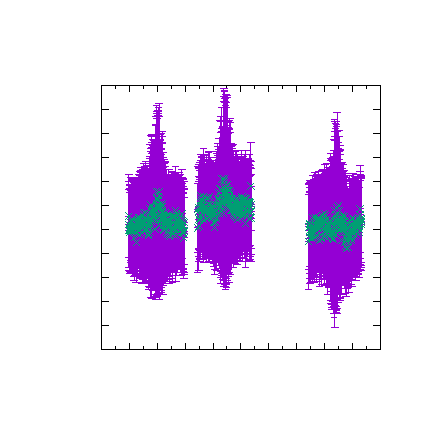
\includegraphics{../images/20160222_NO_fixI0_O3_ts}}%
    \gplfronttext
  \end{picture}%
\endgroup

  \caption{Timeseries of the \ch{NO} and \ch{O3} concentration. The
    three clusters correspond to the three used reaction pathlengths
    $l = 5, 10$ and \SI{15}{\meter}.}
  \label{fig:ts}
\end{figure}
\begin{figure}[H]
  \centering
  % GNUPLOT: LaTeX picture with Postscript
\begingroup
  \makeatletter
  \providecommand\color[2][]{%
    \GenericError{(gnuplot) \space\space\space\@spaces}{%
      Package color not loaded in conjunction with
      terminal option `colourtext'%
    }{See the gnuplot documentation for explanation.%
    }{Either use 'blacktext' in gnuplot or load the package
      color.sty in LaTeX.}%
    \renewcommand\color[2][]{}%
  }%
  \providecommand\includegraphics[2][]{%
    \GenericError{(gnuplot) \space\space\space\@spaces}{%
      Package graphicx or graphics not loaded%
    }{See the gnuplot documentation for explanation.%
    }{The gnuplot epslatex terminal needs graphicx.sty or graphics.sty.}%
    \renewcommand\includegraphics[2][]{}%
  }%
  \providecommand\rotatebox[2]{#2}%
  \@ifundefined{ifGPcolor}{%
    \newif\ifGPcolor
    \GPcolorfalse
  }{}%
  \@ifundefined{ifGPblacktext}{%
    \newif\ifGPblacktext
    \GPblacktexttrue
  }{}%
  % define a \g@addto@macro without @ in the name:
  \let\gplgaddtomacro\g@addto@macro
  % define empty templates for all commands taking text:
  \gdef\gplbacktext{}%
  \gdef\gplfronttext{}%
  \makeatother
  \ifGPblacktext
    % no textcolor at all
    \def\colorrgb#1{}%
    \def\colorgray#1{}%
  \else
    % gray or color?
    \ifGPcolor
      \def\colorrgb#1{\color[rgb]{#1}}%
      \def\colorgray#1{\color[gray]{#1}}%
      \expandafter\def\csname LTw\endcsname{\color{white}}%
      \expandafter\def\csname LTb\endcsname{\color{black}}%
      \expandafter\def\csname LTa\endcsname{\color{black}}%
      \expandafter\def\csname LT0\endcsname{\color[rgb]{1,0,0}}%
      \expandafter\def\csname LT1\endcsname{\color[rgb]{0,1,0}}%
      \expandafter\def\csname LT2\endcsname{\color[rgb]{0,0,1}}%
      \expandafter\def\csname LT3\endcsname{\color[rgb]{1,0,1}}%
      \expandafter\def\csname LT4\endcsname{\color[rgb]{0,1,1}}%
      \expandafter\def\csname LT5\endcsname{\color[rgb]{1,1,0}}%
      \expandafter\def\csname LT6\endcsname{\color[rgb]{0,0,0}}%
      \expandafter\def\csname LT7\endcsname{\color[rgb]{1,0.3,0}}%
      \expandafter\def\csname LT8\endcsname{\color[rgb]{0.5,0.5,0.5}}%
    \else
      % gray
      \def\colorrgb#1{\color{black}}%
      \def\colorgray#1{\color[gray]{#1}}%
      \expandafter\def\csname LTw\endcsname{\color{white}}%
      \expandafter\def\csname LTb\endcsname{\color{black}}%
      \expandafter\def\csname LTa\endcsname{\color{black}}%
      \expandafter\def\csname LT0\endcsname{\color{black}}%
      \expandafter\def\csname LT1\endcsname{\color{black}}%
      \expandafter\def\csname LT2\endcsname{\color{black}}%
      \expandafter\def\csname LT3\endcsname{\color{black}}%
      \expandafter\def\csname LT4\endcsname{\color{black}}%
      \expandafter\def\csname LT5\endcsname{\color{black}}%
      \expandafter\def\csname LT6\endcsname{\color{black}}%
      \expandafter\def\csname LT7\endcsname{\color{black}}%
      \expandafter\def\csname LT8\endcsname{\color{black}}%
    \fi
  \fi
    \setlength{\unitlength}{0.0500bp}%
    \ifx\gptboxheight\undefined%
      \newlength{\gptboxheight}%
      \newlength{\gptboxwidth}%
      \newsavebox{\gptboxtext}%
    \fi%
    \setlength{\fboxrule}{0.5pt}%
    \setlength{\fboxsep}{1pt}%
\begin{picture}(7200.00,5040.00)%
    \gplgaddtomacro\gplbacktext{%
      \csname LTb\endcsname%
      \put(682,704){\makebox(0,0)[r]{\strut{}$0$}}%
      \put(682,1213){\makebox(0,0)[r]{\strut{}$10$}}%
      \put(682,1722){\makebox(0,0)[r]{\strut{}$20$}}%
      \put(682,2231){\makebox(0,0)[r]{\strut{}$30$}}%
      \put(682,2740){\makebox(0,0)[r]{\strut{}$40$}}%
      \put(682,3248){\makebox(0,0)[r]{\strut{}$50$}}%
      \put(682,3757){\makebox(0,0)[r]{\strut{}$60$}}%
      \put(682,4266){\makebox(0,0)[r]{\strut{}$70$}}%
      \put(682,4775){\makebox(0,0)[r]{\strut{}$80$}}%
      \put(814,484){\makebox(0,0){\strut{}$4$}}%
      \put(1563,484){\makebox(0,0){\strut{}$6$}}%
      \put(2311,484){\makebox(0,0){\strut{}$8$}}%
      \put(3060,484){\makebox(0,0){\strut{}$10$}}%
      \put(3809,484){\makebox(0,0){\strut{}$12$}}%
      \put(4557,484){\makebox(0,0){\strut{}$14$}}%
      \put(5306,484){\makebox(0,0){\strut{}$16$}}%
      \put(6054,484){\makebox(0,0){\strut{}$18$}}%
      \put(6803,484){\makebox(0,0){\strut{}$20$}}%
    }%
    \gplgaddtomacro\gplfronttext{%
      \csname LTb\endcsname%
      \put(176,2739){\rotatebox{-270}{\makebox(0,0){\strut{}Concentration [ppb]}}}%
      \put(3808,154){\makebox(0,0){\strut{}Length [m]}}%
      \csname LTb\endcsname%
      \put(5816,4602){\makebox(0,0)[r]{\strut{}0.01\ \si{\liter\per\minute}}}%
      \csname LTb\endcsname%
      \put(5816,4382){\makebox(0,0)[r]{\strut{}0.03\ \si{\liter\per\minute}}}%
      \csname LTb\endcsname%
      \put(5816,4162){\makebox(0,0)[r]{\strut{}0.05\ \si{\liter\per\minute}}}%
      \csname LTb\endcsname%
      \put(5816,3942){\makebox(0,0)[r]{\strut{}0.1\ \si{\liter\per\minute}}}%
      \csname LTb\endcsname%
      \put(5816,3722){\makebox(0,0)[r]{\strut{}0.2\ \si{\liter\per\minute}}}%
      \csname LTb\endcsname%
      \put(5816,3502){\makebox(0,0)[r]{\strut{}0.3\ \si{\liter\per\minute}}}%
    }%
    \gplbacktext
    \put(0,0){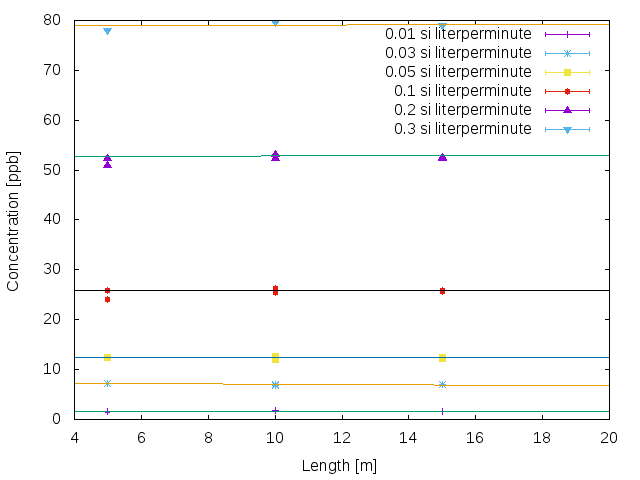
\includegraphics{../images/20160222_NO_fixI0_NO_length}}%
    \gplfronttext
  \end{picture}%
\endgroup

  \caption{\ch{NO} concentration dependence on reaction path
    length. The data points are colored depending on the applied
    \ch{NO} flow. All data points were linearly interpolated. The
    results can also be found in the plot.}
  \label{fig:no-length}
\end{figure}

Comparing next the \ch{NO2} plateaus between multiple pathlengths, we
see that the concentrations seem to coincide. Averaging them and
plotting them over the pathlength we yield Figure~\ref{fig:no-length},
which confirms this assertion. The data points at coresponding flows
were linearly interpolated to make drifts more tangible. The fits are
also plotted in the figure. The interpolation showed that the slope
was undiscernible from zero in each case. At the \SI{5}{\meter}
setting one of the red and one of the violet data points seem to be
off. These two data points correspond to the rising flanks discussed
extensively above. It seems that at these two data points the
equilibrium had not been reached and we averaged too early.

\begin{figure}[htbp]
  \centering
  % GNUPLOT: LaTeX picture with Postscript
\begingroup
  \makeatletter
  \providecommand\color[2][]{%
    \GenericError{(gnuplot) \space\space\space\@spaces}{%
      Package color not loaded in conjunction with
      terminal option `colourtext'%
    }{See the gnuplot documentation for explanation.%
    }{Either use 'blacktext' in gnuplot or load the package
      color.sty in LaTeX.}%
    \renewcommand\color[2][]{}%
  }%
  \providecommand\includegraphics[2][]{%
    \GenericError{(gnuplot) \space\space\space\@spaces}{%
      Package graphicx or graphics not loaded%
    }{See the gnuplot documentation for explanation.%
    }{The gnuplot epslatex terminal needs graphicx.sty or graphics.sty.}%
    \renewcommand\includegraphics[2][]{}%
  }%
  \providecommand\rotatebox[2]{#2}%
  \@ifundefined{ifGPcolor}{%
    \newif\ifGPcolor
    \GPcolorfalse
  }{}%
  \@ifundefined{ifGPblacktext}{%
    \newif\ifGPblacktext
    \GPblacktexttrue
  }{}%
  % define a \g@addto@macro without @ in the name:
  \let\gplgaddtomacro\g@addto@macro
  % define empty templates for all commands taking text:
  \gdef\gplbacktext{}%
  \gdef\gplfronttext{}%
  \makeatother
  \ifGPblacktext
    % no textcolor at all
    \def\colorrgb#1{}%
    \def\colorgray#1{}%
  \else
    % gray or color?
    \ifGPcolor
      \def\colorrgb#1{\color[rgb]{#1}}%
      \def\colorgray#1{\color[gray]{#1}}%
      \expandafter\def\csname LTw\endcsname{\color{white}}%
      \expandafter\def\csname LTb\endcsname{\color{black}}%
      \expandafter\def\csname LTa\endcsname{\color{black}}%
      \expandafter\def\csname LT0\endcsname{\color[rgb]{1,0,0}}%
      \expandafter\def\csname LT1\endcsname{\color[rgb]{0,1,0}}%
      \expandafter\def\csname LT2\endcsname{\color[rgb]{0,0,1}}%
      \expandafter\def\csname LT3\endcsname{\color[rgb]{1,0,1}}%
      \expandafter\def\csname LT4\endcsname{\color[rgb]{0,1,1}}%
      \expandafter\def\csname LT5\endcsname{\color[rgb]{1,1,0}}%
      \expandafter\def\csname LT6\endcsname{\color[rgb]{0,0,0}}%
      \expandafter\def\csname LT7\endcsname{\color[rgb]{1,0.3,0}}%
      \expandafter\def\csname LT8\endcsname{\color[rgb]{0.5,0.5,0.5}}%
    \else
      % gray
      \def\colorrgb#1{\color{black}}%
      \def\colorgray#1{\color[gray]{#1}}%
      \expandafter\def\csname LTw\endcsname{\color{white}}%
      \expandafter\def\csname LTb\endcsname{\color{black}}%
      \expandafter\def\csname LTa\endcsname{\color{black}}%
      \expandafter\def\csname LT0\endcsname{\color{black}}%
      \expandafter\def\csname LT1\endcsname{\color{black}}%
      \expandafter\def\csname LT2\endcsname{\color{black}}%
      \expandafter\def\csname LT3\endcsname{\color{black}}%
      \expandafter\def\csname LT4\endcsname{\color{black}}%
      \expandafter\def\csname LT5\endcsname{\color{black}}%
      \expandafter\def\csname LT6\endcsname{\color{black}}%
      \expandafter\def\csname LT7\endcsname{\color{black}}%
      \expandafter\def\csname LT8\endcsname{\color{black}}%
    \fi
  \fi
    \setlength{\unitlength}{0.0500bp}%
    \ifx\gptboxheight\undefined%
      \newlength{\gptboxheight}%
      \newlength{\gptboxwidth}%
      \newsavebox{\gptboxtext}%
    \fi%
    \setlength{\fboxrule}{0.5pt}%
    \setlength{\fboxsep}{1pt}%
\begin{picture}(7776.00,4320.00)%
    \gplgaddtomacro\gplbacktext{%
      \csname LTb\endcsname%
      \put(682,704){\makebox(0,0)[r]{\strut{}$0$}}%
      \put(682,1076){\makebox(0,0)[r]{\strut{}$10$}}%
      \put(682,1449){\makebox(0,0)[r]{\strut{}$20$}}%
      \put(682,1821){\makebox(0,0)[r]{\strut{}$30$}}%
      \put(682,2193){\makebox(0,0)[r]{\strut{}$40$}}%
      \put(682,2566){\makebox(0,0)[r]{\strut{}$50$}}%
      \put(682,2938){\makebox(0,0)[r]{\strut{}$60$}}%
      \put(682,3310){\makebox(0,0)[r]{\strut{}$70$}}%
      \put(682,3683){\makebox(0,0)[r]{\strut{}$80$}}%
      \put(682,4055){\makebox(0,0)[r]{\strut{}$90$}}%
      \put(814,484){\makebox(0,0){\strut{}$0$}}%
      \put(1543,484){\makebox(0,0){\strut{}$10$}}%
      \put(2273,484){\makebox(0,0){\strut{}$20$}}%
      \put(3002,484){\makebox(0,0){\strut{}$30$}}%
      \put(3732,484){\makebox(0,0){\strut{}$40$}}%
      \put(4461,484){\makebox(0,0){\strut{}$50$}}%
      \put(5191,484){\makebox(0,0){\strut{}$60$}}%
      \put(5920,484){\makebox(0,0){\strut{}$70$}}%
      \put(6650,484){\makebox(0,0){\strut{}$80$}}%
      \put(7379,484){\makebox(0,0){\strut{}$90$}}%
    }%
    \gplgaddtomacro\gplfronttext{%
      \csname LTb\endcsname%
      \put(176,2379){\rotatebox{-270}{\makebox(0,0){\strut{}\ch{NO} Concentration, measured with ICAD [ppb]}}}%
      \put(4096,154){\makebox(0,0){\strut{}\ch{NO} Concentration, calculated [ppb]}}%
    }%
    \gplbacktext
    \put(0,0){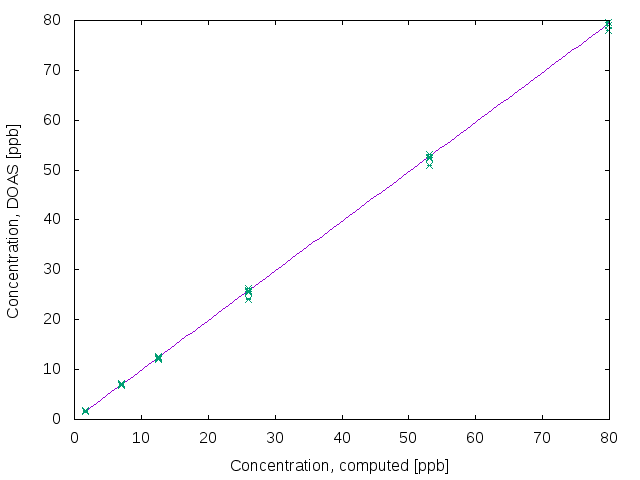
\includegraphics{../images/20160222_NO_fixI0}}%
    \gplfronttext
  \end{picture}%
\endgroup

  \caption{Correlation plot of the computed and the measured \ch{NO}
    concentration.}
  \label{fig:no-calib}
\end{figure}

Since Figure~\ref{fig:no-length} indicated that the measured
concentrations aret pathlength independent (except for the two outliers),
we can use all of them to research the correlation between our
measured concentrations and the ones computed from the flow by
Equation~\eqref{eq:c-flow}. The result can be seen in
Figure~\ref{fig:no-calib} together with a linear regression. The
regression formula yields

\begin{align*}
  y = \num{0.994 \pm 0.002}  \cdot x -\num{0.002 \pm 0.058}.
\end{align*}
Also we end up with a Pearson's r 0.994 which also indicates the high
correlation between the measured and the computed data.

Thus we see that the deviation between the measured and computed
concentration lies in the per mill regime. We see that under these
controlled conditions our converter works and does not introduce
tangible systematic errors. Figure~\ref{fig:ts} implies that a
\SI{10}{\meter} reaction path is sufficient and will therefore be used
for the following experiments.

%%% Local Variables:
%%% mode: latex
%%% TeX-master: "../Bachelor"
%%% End:
